\documentclass[draft]{agujournal2019}
\usepackage{url}
\usepackage{lineno}
\usepackage{soul}

\linenumbers
\draftfalse
\journalname{Earth and Space Science}


\begin{document}

\title{AuroraX, aurorax-api (or pyaurorax?), and aurorax-asilib: a user-friendly auroral all-sky imager analysis framework}

\authors{M. Shumko\affil{1, 2}, B. Gallardo-Lacourt\affil{1,2}, A.J. Halford\affil{1}, E. Donovan\affil{3}, E.L. Spanswick\affil{3}, D. Chaddock\affil{3}, I. Thompson, and K.R. Murphy}

\affiliation{1}{NASA's Goddard Space Flight Center, Greenbelt, Maryland, USA}
\affiliation{2}{Universities Space Research Association, Columbia, Maryland, USA}
\affiliation{3}{University of Calgary, Calgary, Alberta, Canada}

\correspondingauthor{M. Shumko}{msshumko@gmail.com}


\begin{keypoints}
\item AuroraX is an online interface to visualize the aurora and calculate conjunctions
\item aurorax-asilib is a companion Python package for detailed analysis of auroral all-sky imager data 
\item Together, these tools enable effortless end-to-end discovery and analysis of the aurora
\end{keypoints}


\begin{abstract}
Abstract
\end{abstract}


\section*{Plain Language Summary}
\noindent


\section{Introduction}\label{intro}
\textcolor{blue}{
      OUTLINE
      \begin{itemize}
            \item Brief history of ASIs and ASI arrays. Talk about why THEMIS ASI exists. Discuss CANOPUS? Linage.
            \item Breadth of possible science questions that can be answered with aurora image data.
            \item Problem: modern ASI arrays produce an immense volume of data.
            \item Why this software? Aurora ASI data formats very greatly, each with their own caveats. This centralized software package is maintained by the AuroraX team. 
            \item Benefits: Maintained by the AuroraX team so it's usability is of paramount importance
            \item Reduce the barrier to entry into auroral physics. Reduce the technical requirements and  enable rapid discovery of new science.
            \item Instead of case study results, larger statistical behavior will likely appear.
            \item remove the need for scientists needing to write duplicate code to use these popular missions. AS a result, this will enable scientists to dive right into the science and not need to know the details of data management (downloading and loading data, as well as applying routine data processing steps
      \end{itemize}
}

The rapidly increasing amount of imager data, together with unique data formats, significantly burdens space physicists with mondale and duplicated software engineering tasks---download data, load and parse the data correctly, etc. This unnecessary burden can also lead to mistakes in analysis software that may require unnecessary troubleshooting time from the ASI team. The goal of AuroraX is to overcome these drawbacks by providing a set of robust tools that most researchers need to analyze all-sky images. 

We describe our progress towards that goal in this article. First, we showcase the main features of the online AuroraX interface (https://aurorax.space/) such as the conjunction finder and the keogram finder. Second, we describe the aurorax-api, a Python library containing the interface to the AuroraX server to automatically download keograms and identify conjunctions. Third, we describe aurorax-asilib, the Python all-sky imager library. aurorax-asilib provides functions to the download, load, process data, and visualize THEMIS and REGO ASI data. 


\section{Design Philosophy (Principals?)}
\textcolor{blue}{
      OUTLINE
      \begin{itemize}
            \item The primary design philosophy is to offer a robust set of functions that are useful for most researchers studying the aurora. We strived to strike a balance between complicated and user-friendly tools. 
            \item Online keogram and conjunction interface accessible anywhere with internet connection.
            \item Comprehensive ASI data analysis functionality on a PC.
            \item Abstract away data management steps: downloading data, loading data, applying routine data processing steps, and common visualizations.
      \end{itemize}
}

\section{AuroraX}\label{aurorax}
\textcolor{blue}{
      OUTLINE
      \begin{itemize}
            \item What is it?
            \item A highly optimized conjunction search
            \item On-demand keograms
            \item Virtual Observatory
            \item pyaurorax (aurorax-api) to directly access AuroraX services.
            \item Figure 1: a) a screenshot of the nightly keograms, b) screenshot of the conjunction search tool. 
      \end{itemize}
}

\section{aurorax-asilib}\label{aurorax-asilib}
\textcolor{blue}{
      OUTLINE
      \begin{itemize}
            \item What is it? A Python library that helps researchers analyze THEMIS and REGO ASI images.The main functions are summarized in Table 1. It is designed to be simple and runnable on personal machines (relatively low memory usage). We strived to strike a balance between complicated and user-friendly tools.
            \item A table of function names and one sentence to describe their functions.
            \item The large file sizes lead to relatively long processing time. This is a fact that can be partly mitigated by an SSD. 
            \item Plug-in based architecture that allows new ASI arrays to be added and called by the core aurorax-asilib software.
      \end{itemize}
}

aurorax-asilib allows researchers to analyze ASI data on a PC. It provides a set of functions for common data analysis tasks using ASI data. Here we overview the functions and the online documentation has more examples, a tutorial, and a thorough API reference \url{https://aurora-asi-lib.readthedocs.io/}

As we tour the asilib functions, keep in mind that asilib is designed to help you with the lower-level tasks. For example, if you want to load the image data via \verb|asilib.load_image()|, asilib will attempt to download it if it is not already saved on the PC. Likewise, if you call \verb|asilib.plot_keogram()|, it will automatically load (and optionally download) the ASI data for you. Lastly, Figs. 2-\textcolor{red}{X} were made using the code in a Jupyter Notebook that is provided with this article (in both the ipynb and pdf formats).

\subsection{Download and load ASI image and skymap data}
\textcolor{blue}{
      OUTLINE
      \begin{itemize}
            \item Handles the downloading and loading of ASI images. Main design principle: Ultimately, ASI image files consists of time stamps and images, so the asilib functions really only need to return that data
            \item Similarly with skymap calibration files
            \item If a file is already downloaded, you do not need an internet connection to work with the data
      \end{itemize}
}

Let us start with the four functions that download and load ASI image and skymap data: 

\begin{itemize}
      \item \verb|asilib.download_image()|,
      \item \verb|asilib.download_skymap()|,
      \item \verb|asilib.load_image()|, and
      \item \verb|asilib.load_skymap()|
\end{itemize} that are described below.

The \verb|asilib.download_image()| function downloads the level 1 hourly Common Data Format (CDF) files from \url{http://themis.ssl.berkeley.edu/data/themis/thg/l1/asi/} for THEMIS, and \url{http://themis.ssl.berkeley.edu/data/themis/thg/l1/reg/} for REGO. The files are saved in the \verb|asilib.config['ASI_DATA_DIR']| directory that at \verb|~/asilib-data/| be default, and is customizable.

The \verb|asilib.download_skymap()| function downloads all of the skymap files from \url{https://data.phys.ucalgary.ca/sort_by_project/THEMIS/asi/skymaps/} and \url{https://data.phys.ucalgary.ca/sort_by_project/GO-Canada/REGO/skymap/} for a given set of \verb|asi_array_code| and \verb|location_code|. The skymap files are in the Interactive Data Language (IDL) \verb|.sav| file format. Noteworthy is that \verb|asilib| downloads all of the skymap files for a given imager because the skymaps are only valid for a set time period (typically a year; see the logic for \verb|asilib.load_skymap()| that is described below).

As the name implies, \verb|asilib.load_image()| loads into memory and returns the ASI time stamps and images for a specified imager. This function loads both single and multiple images: a single time stamp and image if \verb|time| is provided, and an array of time stamps and images if \verb|time_range| is provided. As previously mentioned,\verb|asilib.load_image()| will try to download an hourly CDF file if it does not exist locally.

\verb|asilib.load_skymap()| is the last noteworthy input function; it loads the relevant skymap file into memory and returns the data in a dictionary. A relevant skymap file is the latest one before the specified \verb|time|. As with \verb|asilib.load_image()|, \verb|asilib.load_skymap()| will attempt to download the skymap functions if they are not already downloaded.

Before we discuss the plotting functions, we emphasize that the \verb|asilib.download_image()| and \verb|asilib.download_skymap()| functions are often unnecessary to call since they are called by \verb|asilib.load_image()| and \verb|asilib.load_skymap()|. However, the download functions are very useful if you need to download ASI image and calibration data in bulk---useful to analyze data offline, for example.

\subsection{Plotting single images}

The \verb|asilib| provides two ways to plot a single ASI image:

\begin{itemize}
      \item \verb|asilib.plot_fisheye()| and
      \item \verb|asilib.plot_map()|.
\end{itemize}

One common way to visualize all-sky images is with \verb|asilib.plot_fisheye()|. It plots the raw ASI images oriented with North at the top and East to the right of each image. The term fisheye comes from the fisheye lens that expands the imager's field of view to nearly $180^\circ$. For reference, the \verb|azel_contours| keyword argument superposes contours of elevation and azimuth in the fisheye image. Figure \ref{fig2}a,c show an example of an auroral arc observed concurrently by the THEMIS and REGO ASIs stationed at Rankin Inlet (RANK). If you don't override the parameters, the color map is automatically chosen: black-to-white for THEMIS and black-to-red for REGO. Also the color scale is dynamically calculated using percentile logic described in the documentation.

Another common way to visualize images is by projecting the fisheye image onto a geographic map using \verb|asilib.plot_map()|. asilib uses the skymap files to map each pixel's vertices to a (latitude, longitude) point at an assumed aurora emission altitude (typically 110 km for THEMIS and 230 km for REGO). Figure \ref{fig2}b,d show the fisheye images mapped to 110 km altitude. By default, pixels that look at $< 10^\circ$ elevations are not mapped due to the stretching of pixels closest to the horizon. And lastly, \verb|asilib.plot_map()| provides default map styles that can be overwritten by your custom \verb|cartopy| map passed in via the \verb|ax| keyword argument.

\begin{figure}
      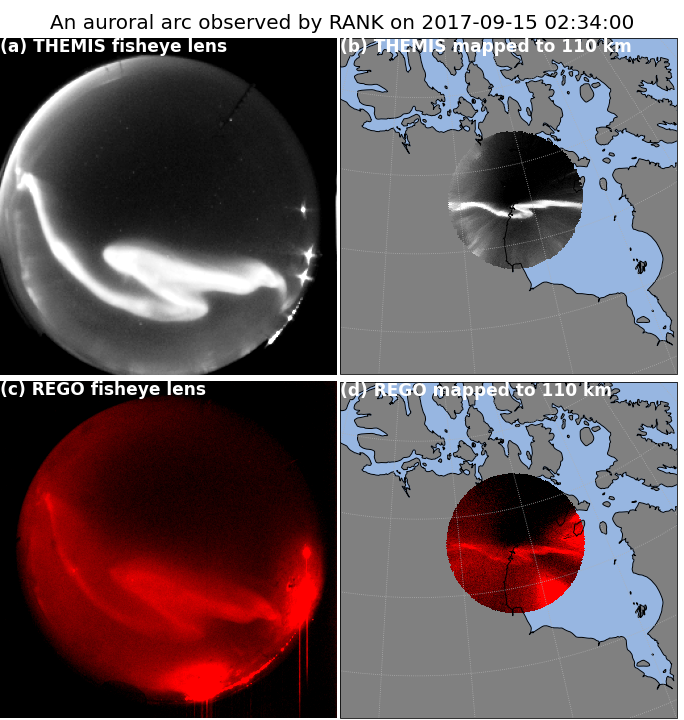
\includegraphics[width=\textwidth]{figures/fig2.png}
      \caption{ASI image of an auroral arc taken simultaneously by the REGO and THEMIS imagers at Rankin Inlet, Canada. Panels and a and c show the raw fisheye lens view, while panels b and d show the same images projected to the 110 km assumed aurora emission altitude. Only the pixels with $>10^\circ$ elevation are plotted.}
      \label{fig2}
\end{figure}

\subsection{Keograms}
\textcolor{blue}{
      OUTLINE
      \begin{itemize}
            \item Figure 3: A keogram for a full night. (REGO)
      \end{itemize}
}

A ubiquitous way to visualize ASI images and identify different types of aurora is with keograms---an image of pixel intensity as a function of latitude and time. Typically, they are assembled by slicing and concatenating pixels that are oriented North-South through zenith (or through a custom path such a path of a stellite) from each image. Keograms are an essential tool that compress the information contained in hours of images into one plot. Objects in the sky such as auroral arcs, pulsating aurora, substorms, clouds, the moon, etc. all have unique keogram signatures that allow you to quickly classify what the imager observed. 

You can make a keogram using the \verb|asilib.plot_keogram()| function (that in turn calls \verb|asilib.keogram()|). Similar to \verb|asilib.plot_map()|, \verb|asilib.plot_keogram()| takes an optional \verb|map_alt| keyword argument. If it is not provided, the keogram's vertical axis is pixel index, but if a valid map altitude is provided, the vertical axis is geographic latitude. To minimize the PC's memory usage, \verb|asilib.keogram()| loads image data using \verb|asilib.load_image_generator()| that processes one image file at a time. The keogram shown in Fig. \ref{fig3} shows the dynamic nature of the aurora. Furthermore, the latitude  mapping transformation between panels a and b is substantial---low elevation pixels map to much wider sections of latitude as compared to the pixels near zenith.

\begin{figure}
      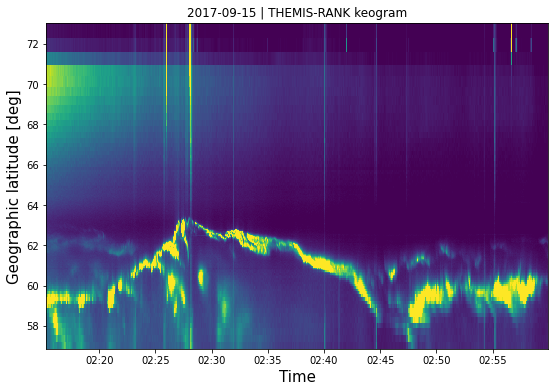
\includegraphics[width=\textwidth]{figures/fig3.png}
      \caption{A full-night keogram showing the dynamic aurora observed at Gillam, Canada. Panel a shows the unmapped keogram with the pixel index vertical axis, while panel b shows the latitude of the pixels mapped to 110 km altitude.}
      \label{fig3}
\end{figure}


\subsection{Creating ASI movies}
\textcolor{blue}{
      OUTLINE
      \begin{itemize}
            \item Basic fisheye animation
            \item Basic map animation (need to add functionality)
            \item Using co-routines to superpose data onto images (extensively used for conjunctions).
            \item Reference SI movie 1.
      \end{itemize}
}

You can easily animate ASI fisheye images using \verb|asilib.plot_fisheye_movie()|. It first saves png images in a unique subfolder in the \verb|~/asilib-data/movies/frames/| folder, and then animates them using the \verb|ffmpeg| library. Movie S1 in the supporting information (SI) document shows an example of \textcolor{red}{X}. \textcolor{red}{Add} \verb|asilib.plot_map_movie()|?

Animating raw fisheye images is somewhat limiting, thus \verb|asilib| also includes \verb|asilib.plot_movie_generator()| (technically a coroutine) to create a stream of customizable ASI images. You can then modify each image before \verb|asilib.plot_movie_generator()| saves the image frame and combines it into a movie. A common use of this generator function is to superpose your data onto each ASI image, as for a conjunction described in Section \ref{satellite_conjunction}.

\subsection{ASI analysis tools}
\textcolor{blue}{
      OUTLINE
      \begin{itemize}
            \item lla2azel
            \item lla2footprint (requires IRBEM)
            \item area2pixels
      \end{itemize}
}

\subsection{An example: a satellite-ASI conjunction}\label{satellite_conjunction}
\textcolor{blue}{
      OUTLINE
      \begin{itemize}
            \item Combine everything above into an example showing where the footprint of a LEO satellite is, and what 
            \item Figure 4: A conjunction montage and a time series
            \item (Implement an Imager.conjunction function)
            \item Reference movie S2
      \end{itemize}
}

\section{Quality Assurance}
\textcolor{blue}{
      OUTLINE
      \begin{itemize}
            \item asilib on GitHub. unit and integration tests run automatically before every release.
            \item THEMIS and REGO data formats are set and won't change.
      \end{itemize}
}

\section{Future Development}
\textcolor{blue}{
      OUTLINE
      \begin{itemize}
            \item Switch from CDF to pgm files.
            \item Support more ASI arrays such as TREx
            \item Community challenge. This package is made for the space physics community, so we will seek feedback (in the form of issues and bugs) that are discovered during a community challenge time period. 
            \item Combine into a class architecture to share data.
      \end{itemize}
}
While aurorax-asilib is feature complete, we plan to keep developing it.

\section{Conclusion}

\textcolor{blue}{
      OUTLINE
      \begin{itemize}
            \item AuroraX, aurorax-api, and aurorax-asilib tools provide the science community with a simple and a robust set of analysis tools
            \item Enable system-level science to be easily done
            \item Quickly sift through an immense volume of data to uncover new physics
            \item This is an end-to-end solution
            \item Plan to add support for other ASI arrays and satellites
            \item Help promote a uniform ASI data format for future cameras
      \end{itemize}
}

\acknowledgments
We are thankful for the engineers and scientists who made AuroraX, THEMIS ASI, and REGO ASI projects possible. M. Shumko and B. Gallardo-Lacourt acknowledge the support provided by the NASA Postdoctoral Program at the NASA’s Goddard Space Flight Center, administered by Universities Space Research Association under contract with NASA. The THEMIS and REGO ASI data is available from \url{https://data.phys.ucalgary.ca/}.

% \bibliography{refs.bib}

\end{document}